\documentclass[conference]{IEEEtran}

\usepackage{cite}
\usepackage{amsmath,amssymb,amsfonts}
\usepackage{algorithmic}
\usepackage{graphicx}
\usepackage{textcomp}
\usepackage{xcolor}
\def\BibTeX{{\rm B\kern-.05em{\sc i\kern-.025em b}\kern-.08em
    T\kern-.1667em\lower.7ex\hbox{E}\kern-.125emX}}
\graphicspath{ {./images/} }

\begin{document}

\title{Frequency Hopping and Pattern Recognition}

\author{\IEEEauthorblockN{Bailey Fiscus}
\IEEEauthorblockA{\textit{Electrical and Computer Engineering Department} \\
\textit{Stevens Institute of Technology}\\
Hoboken, United States \\
bfiscus@stevens.edu}
}

\maketitle

\begin{abstract}
Frequency hopping has many advantages for wireless communication, including security and resistance to interference.
Due to this, frequency hopping is common among wireless systems.
There is much study in detecting frequency hopping patterns, thus allowing a third-party to eavesdrop.
This paper will explore a method for determining the frequency and duration pattern for an unknown frequency hopping system.
\end{abstract}

\begin{IEEEkeywords}
wireless, frequency hopping, pattern recognition, simulation
\end{IEEEkeywords}

\section{Introduction}
Wireless communication is subject to several issues not faced by wired communication.
Since wireless communication requires broadcasting a signal over a given frequency, any receiver tuned to that frequency will be able to listen to messages.
Additionally, interference can occur in part of the frequency band causing disruption and communication errors.
To alleviate these issues, many modern wireless communications implement frequency hopping.

Frequency hopping involves sending a message over different frequencies in the band for a various duration.
First, the band is split up into a determined number of channels. Each channel has a central frequency, as well as a band gap to avoid interference among the channels.
The sender and receiver will alternate channels in the band for a predetermined duration (often a length of time correlated to a certain number of frames).
Fig. 1 shows this concept with Frequency Hopping Spread Spectrum.

%\begin{figure}[!t]
%\centering
\begin{center}
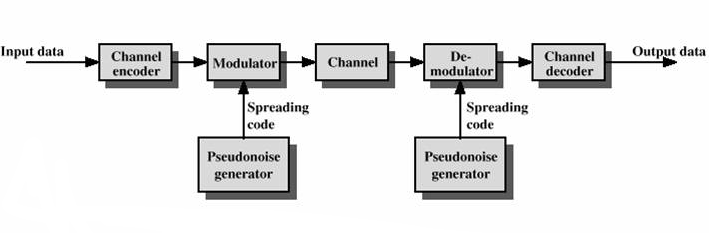
\includegraphics[width=2.5in]{fhss.png}
\text{Fig. 1 Frequency Hopping Spread Spectrum block diagram}
\end{center}
%\label{fig_sim}
%\end{figure}

This predefined, ordered mapping of frequency and duration is referred to as the frequency hopping pattern (FHP).
Using a FHP, transmission errors due to interference are lessened since the affected channel will only be transmitted on for a brief period.
Additionally, it is more difficult for an attacker to listen to communication on a frequency hopping system if they do not know the FHP.

This concept is incredibly common, to the point of ubiquity.
It is used in both commercial and military environments.
Some notable examples of frequency hopping in daily life are IEEE's 802.11 standard (Wi-Fi), and bluetooth.

There is much study into the field of pattern recognition for FHPs.
By monitoring a given band, it is possible to derive the FHP.
Once the pattern is obtained, eavesdropping on the communication becomes possible.
The third-party need only tune its receiver to the appropriate channel during the known duration.
Alternatively, one can follow the FHP and jam each frequency [3] to completely disrupt communication.
This particular application has its use for military operations.

An interesting and common complication with detecting a FHP over a frequency band is the case of multiple sender with different FHP sending at once.

\section{Problem Statement}

The goal of this project is to be able to model a wireless system which uses frequency hopping, and then detect the FHP with little to no prior knowledge on the end of the detector.
This will involve some mathematical modeling, as well as a programming simulation to test the results.
As such, there are several important steps necessary to complete this project.

First, we will need to find a way to model the wireless medium.
At minimum, the model must be able to simulate communication over several channels, with the ability for receivers to listen on different channels (not just the one being transmitted over).

After we have created our model, we will create a way to simulate communication over the virtual, wireless medium.
To start, this probably not be actual symbols being transmitted.
Rather, it will likely be a binary operation in which a given channel is either (1) being transmitted on or (0) not.

Next, we will need to create and distribute a shared FHP between the sender, and receiver.
This FHP will have its own set of constraints and assumptions.
The two most notable will be the maximum transmission duration, and the number of channels.

Then, we will need to create a pattern detection scheme for use with an eavesdropping third-party.
This will be the mathematical side of the project.
It is by this step, that we will need to have our medium and communication completely ironed out.
Prior to completion of those steps, the model will have little to no real-world value.

Finally, we will implement the scheme and determine the correct FHP.

\section{Preliminary Ideas}
This project is split into the aforementioned parts.
We will discuss them in the order in which they were introduced: first the simulation, then the pattern detection.
First, however, we will explore the current assumptions and thoughts I have about the simulation.

First, the simulation should be real time.
A transmission duration of 50us should take 50us (or close to it).
This is done just to increase potential real-world application.
In practice, the virtual system could operate at speeds orders of magnitude faster than its real-world counterpart.
However, this has many potential pitfalls and so we will make this a requirement.

Additionally, this simulation will work with discrete frequency values, or more likely just numbered channels.
This is to remove unfortunate difference in the discrete world of the computer and a real wireless system.
As an example, setting the discrete receiver to listen to the third channel on the 2.4Hz band could easily result in issues regarding \textit{double} values in C++.
This same issue is not as present in analog systems, where the receiver would pick up communication within some threshold from the center frequency.

Finally, the sender will transmit constantly and indefinitely.
To make detection more straightforward (at least for now) the sender should not stop sending.
In a real system, the sender will stop transmitting if it has nothing to say, but this reality makes detecting the correct pattern much more difficult.
Also, the communication would then need to be random and so the performance of the detector could be affected by chance.

\subsection{Implementation in C++}
To implement the model in code, I have chosen to use C++.
This was done to allow possible integration with known communication protocols in the future.
Additionally, C++ will allow fine control over timed events such as delays when listening to a channel, and duration of the transmission.
At present, the entire model contains only four classes.
We will now explore each class to see how they will allow us to adequately simulate a real wireless system. 

\subsubsection{Medium}
This class models the functionality of the actual communication medium.
For this project, the medium which is being modeled is wireless communication.
Originally, I considered using actual \textit{double} values to represent every possible frequency.
This seemed overly-complex to start with, so instead the medium will have a finite number of channels for communication.
Additionally, the medium only accepts one communication at a time.
In the coming weeks I may change this to allow communication on multiple channels (possibly by multiple senders) but that is dependent on the progress made with the detector.
The medium will be shared among all senders and receivers.
Thus, much consideration will be given to thread safety, as each communication device will need to separately operate with the medium in real-time.

\subsubsection{PatternGenerator}
The \textit{PatternGenerator} class is responsible for generating the FHP.
This pattern is shared with the \textit{Sender}, possibly a \textit{reciever}, and is meant to be derived by the \textit{PatternDetector}.
For a given number of channels, and the minimum and maximum time units, a psuedo-random, ordered \textit{vector} of \textit{pairs} is created.
The \textit{pair} consists of the channel to transmit on, and the duration to transmit for.
Since the pattern is a predetermined, finite sequence, it will be shared in its entirety rather than sharing (as an example) a seed or key for generating the pattern.

\subsubsection{Sender}
The \textit{Sender} class uses the generated pattern to continuously transmit over the medium.
An important note is that there are no actual communications sent at present.
Instead, the \textit{Sender} updates \textit{Medium} with the channel that should be considered active.
After the corresponding duration has elapsed, the \textit{Sender} updates the \textit{Medium} that the channel is no longer active.
This continues for the entire FHP, and loops indefinitely.
As noted above, the communication is also entirely simulated.
There are no symbols or bits being sent, rather a binary state of the channel.

\subsubsection{PatternDetector}
The \textit{PatternDetector} class must derive the FHP by only interfacing with the Medium.
The only operation available to it is polling the Medium to determine if the given channel is active.
Using just this, it should be able to implement the mathematical model, and ultimately arrive at the correct FHP.
There are some hurdles already for this particular item.
Since there is currently no minimum listening time, the detector knows immediately after the poll if the channel is active.
Due to this, the detector can currently monitor all channels significantly faster than the shortest random duration.
Until more realistic constraints are set, determining the pattern will be trivial.

The \textit{Sender} and \textit{PatternDetector} operate on different threads.
They both have \textit{pointers} to the shared \textit{Medium} object.
This object has been constructed to be thread-safe, and allow both objects to separately interact with it.
If more senders are added in the future, this thread-safety will need to be revisited as sending over a channel is current not thread-safe.

\subsection{Pattern Detection Mathematical Model}
Although there has been thought about the detection model, there have been no major decisions yet.
This will be done following the completion of the simulation and attached constraints/ assumptions.
Before the exact functionality of the simulation is determined, detecting the FHP will be trivial.
This is due to the real-time waiting at each entry of the pattern.
As an example, waiting for 125ms would be more than enough time for the detector thread to sufficiently check each possible channel.
To create a more realistic simulation (and thus more useful model), more research must be done into limitations of real wireless communication.

\begin{thebibliography}{00}

\bibitem{b1} Y. Wang, Y. Lin, and X. Chi, `` Parameter Estimation Method of Frequency Hopping Signal Based On Sparse Time-frequency Method,'' 2018 IEEE 23rd International Conference on Digital Signal Processing (DSP), Nov. 2018.

\bibitem{b2} K.-G. Lee and S.-J. Oh, “Detection of Fast Frequency-Hopping Signals Using Dirty Template in the Frequency Domain,” IEEE Wireless Communications Letters, vol. 8, no. 1, pp. 281–284, Feb. 2019.

\bibitem{b3} X. Fan and Z. Tan, “Simulink Implementation of Frequency-hopping Communication System and Follower Jamming,” 2018 IEEE International Conference on Automation, Electronics and Electrical Engineering (AUTEEE), Nov. 2018. 

\bibitem{b4} X. Ning, S. Peng, and Z. Wang, “A Novel Anti-interference Scheme of Message-Driven Frequency Hopping Systems,” 2020 IEEE 3rd International Conference on Information Systems and Computer Aided Education (ICISCAE), 2020. 

\end{thebibliography}

\end{document}
